\section{Question}

Let $X$ and $Y$ be independent and exponentially distributed with rates $\lambda_1 = 1$ and $\lambda_2 = 2$ respectively.
\begin{exercise}[0.5]
Find the joint PDF $f(x,y)$ of $X$ and $Y$.
\begin{solution}
    Since $X$ and $Y$ are independent, their joint PDF is the product of their marginal PDFs. This gives:
    \begin{align*}
        f(x,y) = (1e^{-1x})(2e^{-2y}) = 2e^{-x-2y}
    \end{align*} \\
    \textit{One mistake, zero points}
\end{solution}
\end{exercise}

\begin{exercise}[0.5]
Show that $\int_{-\infty}^\infty \int_{-\infty}^\infty f(x,y) \d x \d y = 1$.
\begin{solution}
    Calculating this integral gives:
    \begin{align*}
      \int_{-\infty}^\infty \int_{-\infty}^\infty f(x,y) \d x \d y =& \int_0^\infty \int_0^\infty 2e^{-x-2y} \d x \d y \\
      =& \int_0^\infty 2e^{-2y)}[-e^{-x}]_0^\infty \d y \\
      =& \int_0^\infty 2e^{-2y} \d y \\
      =& \int_0^\infty h(y) \d y \\
      =& 1
    \end{align*}
    Where $h(y)$ is the PDF of $Y$. \\
    \textit{One mistake, zero points}
\end{solution}
\end{exercise}

\begin{exercise}[3]
Find $\E{|X-Y|}$, i.e., the expected distance between $X$ and $Y$.
\begin{solution}
    Similar to example 7.2.2., we get that by 2D LOTUS:
    \begin{align*}
    \E{|X-Y|} =& \int_{-\infty}^\infty \int_{-\infty}^\infty |x-y| f(x,y) \d x \d y \\
    =& \int_0^\infty \int_y^\infty (x-y)  (2e^{-x-2y}) \d x \d y + \int_0^\infty \int_0^y (y-x) (2e^{-x-2y}) \d x \d y \\
    =& \int_0^\infty \left( [(x-y) \cdot -2e^{-x-2y}]_y^\infty - \int_y^\infty - 2e^{-x-2y} \d x \right) \d y \\ &\;\;+ \int_0^\infty  \left( [(y-x) \cdot -2e^{-x-2y}]_0^y - \int_0^y 2e^{-x-2y} \d x \right) \d y \\
    =& \int_0^\infty  [-2e^{-x-2y}]_y^\infty \d y + \int_0^\infty 2y e^{-2y} - [-2e^{-x-2y}]_0^y  \d y \\
    =& \int_0^\infty  2e^{-3y} \d y + \int_0^\infty 2y e^{-2y} + 2e^{-3y} - 2e^{-2y} \d y \\
    =&  \left[-\tfrac23 e^{-3y}\right]_0^\infty + \left[-y e^{-2y} + \tfrac12 e^{-2y} -  \tfrac23 e^{-3y} + e^{-2y}\right]_0^\infty \\
    =& \tfrac23 + \tfrac12 + \tfrac23 - 1
    = \tfrac{5}{6}.
    \end{align*}\\
\textit{One point for writing down the integral correctly using LOTUS and splitting it up correctly. Two points for the computations.}
\end{solution}
\end{exercise}
\noindent Consider the following code:
\begin{minted}{python}
import numpy as np
np.random.seed(3)

num = 500

x = np.random.normal(loc = 50, scale = 200, size = num)

result2 = np.zeros(num)
for i in range(0,num):
    result2[i] = ((x[i]-50)/200)**2

probs = np.arange(0,num)/num
result2 = np.sort(result2)
y = np.random.chisquare(df = 1, size = num)
y = np.sort(y)
plt.plot(result2, probs)
plt.plot(y, probs)
plt.show()

\end{minted}

\begin{exercise}[1]
What does the code above do and why would you expect to get the graph below as output?
\begin{figure}[H]
    \centering
    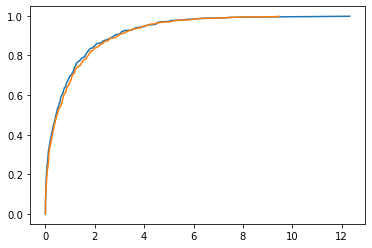
\includegraphics[scale = 0.5]{examplot.png}
\end{figure}
\begin{solution}
It loads the required packages and creates one sample with 500 observations from a $\mathcal{N}(50, 200)$-distribution. Then for all observations it standardizes and takes the square. The empirical CDF of the standardized values is plotted against the PDF of a sample from a chi-square distribution with 1 degree of freedom. It can be seen they look very much alike. This is expected as for $Z \sim \mathcal{N}(0,1)$ we have $Z^2 \sim \chi^2_1$. \\
\textit{0.5 points for mentioning data is standardized, 0.5 points for mentioning a squared standard normal r.v. is chi-square.}
\end{solution}
\end{exercise}
